\documentclass[11pt]{article}
\usepackage{graphicx}
\usepackage{geometry}

\geometry{
	left=25mm,
	right=25mm,
	top=25mm,
	bottom=25mm,
}
\begin{document}
	
	\begin{center}
		\textbf{ASSIGNMENT 7}
	\end{center}
	\textbf{AIM:}
	Implement Naive Bayes for Concurrent/Distributed application. Approach should handle
	categorical and continuous data \\ 
	
	
	\noindent \textbf{OBJECTIVE:}
	\begin{itemize}
		\item To understand basic concept of naive bayes classifier.
		\item To implement naive bayes classifier to predict work type for a person with given attributes.
	\end{itemize}
	
	\noindent \textbf{SOFTWARE REQUIREMENTS:}
	\begin{itemize}
		\item Linux Operating System
		\item Java Compiler
		\item Weka Tool
		\item Eclipse IDE
	\end{itemize}•
	
	\noindent \textbf{MATHEMATICAL MODEL:} \\
	Consider a following set theory notations related to a program. The mathematical model M for
	Naive Bayes classifier is given as below, \\
	M={S,So,A,G} \\
	Where, \\
	S=State space.i.e All prior probabilities to calculate probability of X being a \\
	part of class ‘c’ \\
	So= Initial State.i.e Training set of tuple \\
	A=Set of Actions/Operators.i.e with given dataset predicting the work type
	for a person with give parameters. \\
	G=Goal state.In this case predicting accurate work type for a person. \\
	
	\noindent \textbf{THEORY:} \\
	\paragraph{}
	Naive Bayes Classifier :
	The Naive Bayes classifier is a simple probabilistic classifier which is based on Bayes
	theorem with strong and nave independence assumptions. It is one of the most basic text
	classification techniques with various applications in email spam detection, personal email
	sorting, document categorization, language detection and sentiment detection.
	
	\begin{center}
		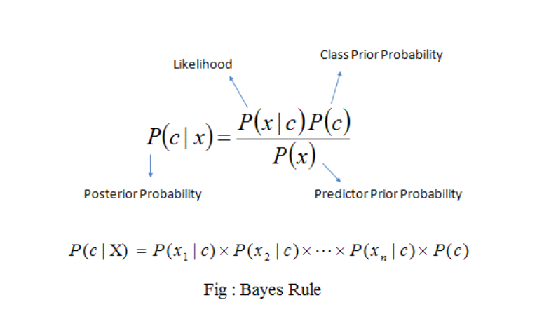
\includegraphics{204/Assign7(naive_bayes)/image1.png}
	\end{center}•
	
	\paragraph{}
	You can use Naive Bayes when you have limited resources in terms of CPU and
	Memory. Moreover when the training time is a crucial factor, Naive Bayes comes handy since it
	can be trained very quickly.
	\paragraph{}
	Let X be a data tuple. In Bayesian terms, X is considered evidence. As usual, it is described by
	measurements made on a set of n attributes. Let H be some hypothesis, such as that the data tuple
	X belongs to a specified class C. For classification problems, we want to determine P(H|X), the
	\paragraph{}
	probability that the hypothesis H holds given the evidence or observed data tuple X.
	The Bayes Naive classifier selects the most likely classification V nb given
	the attribute values a1, a2,... a n .This results in: \\
	
	$V nb =argmax vjEv P( V j )πP( ai|vj )$ \\
	
	We generally estimate P( ai|vj ) using m-estimates: \\
	
	$P( ai|vj ) = f (x) = (nc+mp )/(n+m )$ \\
	
	
	where: \\
	n = the number of training examples for which v = vj \\
	nc = number of examples for which v = vj and a = ai \\
	2p = a priori estimate for P( ai|vj ) \\
	m = the equivalent sample size \\
	
	
	\noindent \textbf{Naive bayes : Car Theft Example} \\
	Attributes are Color, Type, Origin, and the subject, stolen can be either
	yes or no. \\
	1. data set
	
	
	
\includegraphics{204/Assign7(naive_bayes)/image2.png}
	
	\noindent 2. Training example : \\ \\
	We want to classify a Red Domestic SUV. Note \\
	there is no example of a Red Domestic SUV in our data set. Looking \\
	back at equation (2) we can see how to compute this. We need to calculate
	the probabilities. \\
	P(Red|Yes), P(SUV|Yes), P(Domestic|Yes) , \\
	P(Red|No) , P(SUV|No), and P(Domestic|No) \\
	and multiply them by P(Yes) and P(No) respectively . We can estimate these values using
	equation (3). \\
	Looking at P(Red|Yes), we have 5 cases where vj = Yes , and in 3 of those cases ai = Red. So for
	P(Red|Yes), n = 5 and nc = 3. Note that all attribute are binary (two possible values).   \\
	We are
	assuming no other information so, p = 1 / (number-of-attribute-values) = 0.5 for all of our
	attributes. Our m value is arbitrary, (We will use m = 3) but consistent for all attributes. Now we
	simply apply eqauation (3) using the precomputed values of n , nc, p, and m. \\ \\
	
	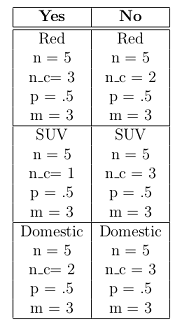
\includegraphics{204/Assign7(naive_bayes)/image3.png} \\ \\
	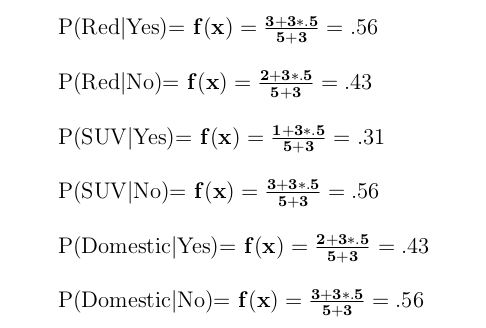
\includegraphics{204/Assign7(naive_bayes)/image4.png} \\ \\
	
	
	We have P(Yes) = .5 and P(No) = .5, so we can apply equation (2). \\
	For v = Yes, we have \\
	P(Yes) * P(Red | Yes) * P(SUV | Yes) * P(Domestic|Yes) \\
	= .5 * .56 * .31 * .43 = .037 \\
	and for v = No, we have \\
	P(No) * P(Red | No) * P(SUV | No) * P (Domestic | No) \\
	= .5 * .43 * .56 * .56 = .069 \\
	Since 0.069 > 0.037, our example gets classified as ‘NO’ \\
	
	\textbf{ Types of Probabilities:}
	1. Prior Probability : \\
	Prior probabilities represent what we originally believed before new evidence
	is uncovered.New information is used to produce updated probabilities
	and is a more accurate measure of a potential outcome.It can
	be represented as,P(x) \\
	2. Conditional Probability : \\
	A conditional probability is the probability of an event, given some
	other event has already occured.It can be represented as,P(x|y)
	3. Posterior Probability : \\
	The posterior probability is the probability of event A occurring given
	that event B has occured.In other words,Posterior probability is the
	probability of the parameters given the evidence.It can be represented
	as,P(z|x) \\
	
	\textbf{CONCLUSION :}
	Thus, we have implemented Naive Bayes for Concurrent/Distributed application
	
	\begin{center}
		\begin{tabular}
			{|c|c|c|c|c|}\hline
			{\bf Roll No.}		&{\bf Name of Student}	&{\bf Date of Performance}  				&{\bf Date of Submission}	&{\bf Sign.}  \\    \hline
			BECOC357	& Sunny Shah  & 28 / 09 / 2017		& 05 / 10 / 2017		&  \\ \hline
		\end{tabular}\\ 
	\end{center}
	
\end{document}
